%%%%%%%%%%%%%%%%%%%%%%%%%%%%%%%%%%%%%%%%%
% Beamer Presentation
% LaTeX Template
% Version 1.0 (10/11/12)
%
% This template has been downloaded from:
% http://www.LaTeXTemplates.com
%
% License:
% CC BY-NC-SA 3.0 (http://creativecommons.org/licenses/by-nc-sa/3.0/)
%
%%%%%%%%%%%%%%%%%%%%%%%%%%%%%%%%%%%%%%%%%

%----------------------------------------------------------------------------------------
%	PACKAGES AND THEMES
%----------------------------------------------------------------------------------------

\documentclass{beamer}

\mode<presentation> {

% The Beamer class comes with a number of default slide themes
% which change the colors and layouts of slides. Below this is a list
% of all the themes, uncomment each in turn to see what they look like.

%\usetheme{default}
%\usetheme{AnnArbor}
%\usetheme{Antibes}
%\usetheme{Bergen}
%\usetheme{Berkeley}
%\usetheme{Berlin}
%\usetheme{Boadilla}
%\usetheme{CambridgeUS}
%\usetheme{Copenhagen}
%\usetheme{Darmstadt}
%\usetheme{Dresden}
%\usetheme{Frankfurt}
%\usetheme{Goettingen}
%\usetheme{Hannover}
%\usetheme{Ilmenau}
%\usetheme{JuanLesPins}
%\usetheme{Luebeck}
\usetheme{Madrid}
%\usetheme{Malmoe}
%\usetheme{Marburg}
%\usetheme{Montpellier}
%\usetheme{PaloAlto}
%\usetheme{Pittsburgh}
%\usetheme{Rochester}
%\usetheme{Singapore}
%\usetheme{Szeged}
%\usetheme{Warsaw}

% As well as themes, the Beamer class has a number of color themes
% for any slide theme. Uncomment each of these in turn to see how it
% changes the colors of your current slide theme.

%\usecolortheme{albatross}
%\usecolortheme{beaver}
%\usecolortheme{beetle}
%\usecolortheme{crane}
%\usecolortheme{dolphin}
%\usecolortheme{dove}
%\usecolortheme{fly}
%\usecolortheme{lily}
%\usecolortheme{orchid}
%\usecolortheme{rose}
%\usecolortheme{seagull}
%\usecolortheme{seahorse}
%\usecolortheme{whale}
%\usecolortheme{wolverine}

%\setbeamertemplate{footline} % To remove the footer line in all slides uncomment this line
%\setbeamertemplate{footline}[page number] % To replace the footer line in all slides with a simple slide count uncomment this line

%\setbeamertemplate{navigation symbols}{} % To remove the navigation symbols from the bottom of all slides uncomment this line
}

\usepackage{graphicx} % Allows including images


\begin{document}

\section{Multi-Output Prediction Model}

\begin{frame}{Shared Forest}

\end{frame}

\section{Simulation Results} 

\subsection{Binary/Continuous} 

\begin{frame}{Predicting Individual $Y^*$ }
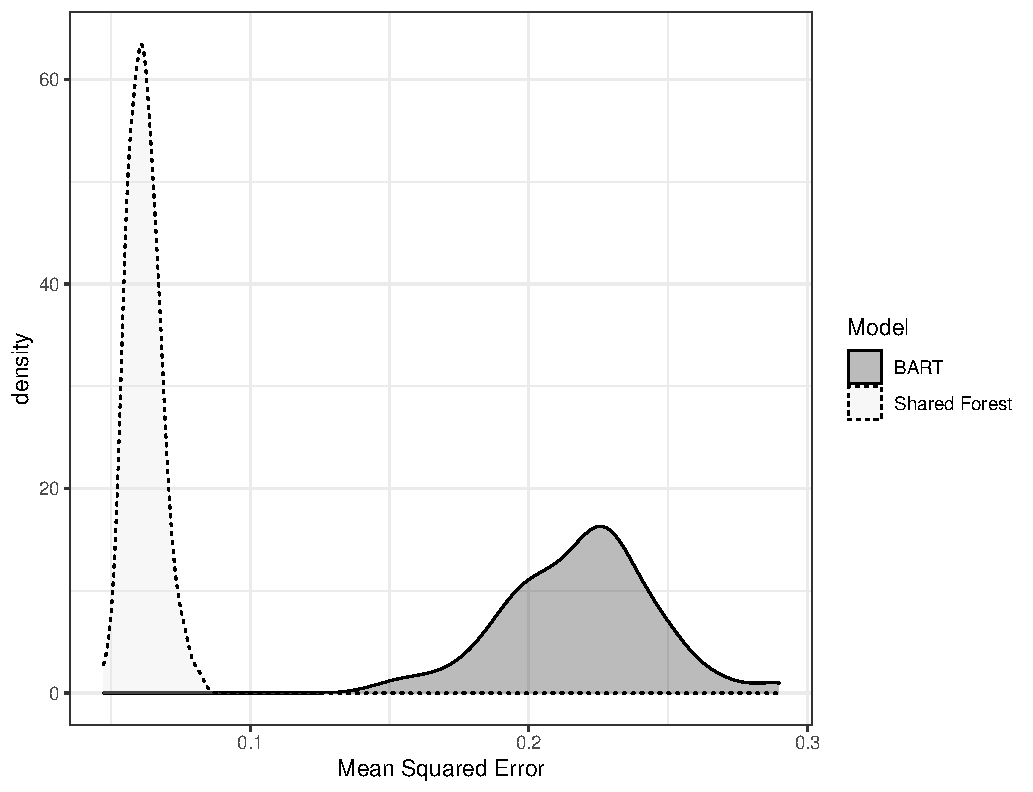
\includegraphics[width = .9\linewidth]{continuous_sim_results_ind_y.pdf}
\end{frame}

\begin{frame}{Predicting Individual $\delta*$}
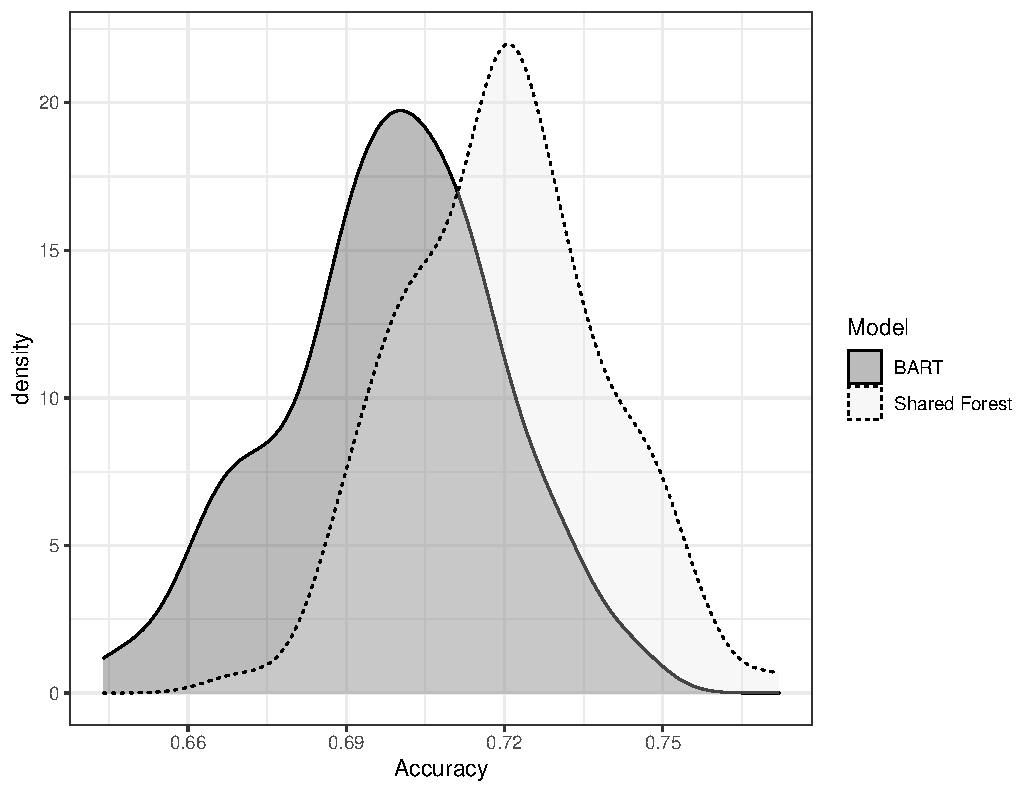
\includegraphics[width = .9\linewidth]{continuous_sim_results_ind_delta.pdf}
\end{frame}


\begin{frame}{Predicting $E(Y^* \mid \delta^*)$ }
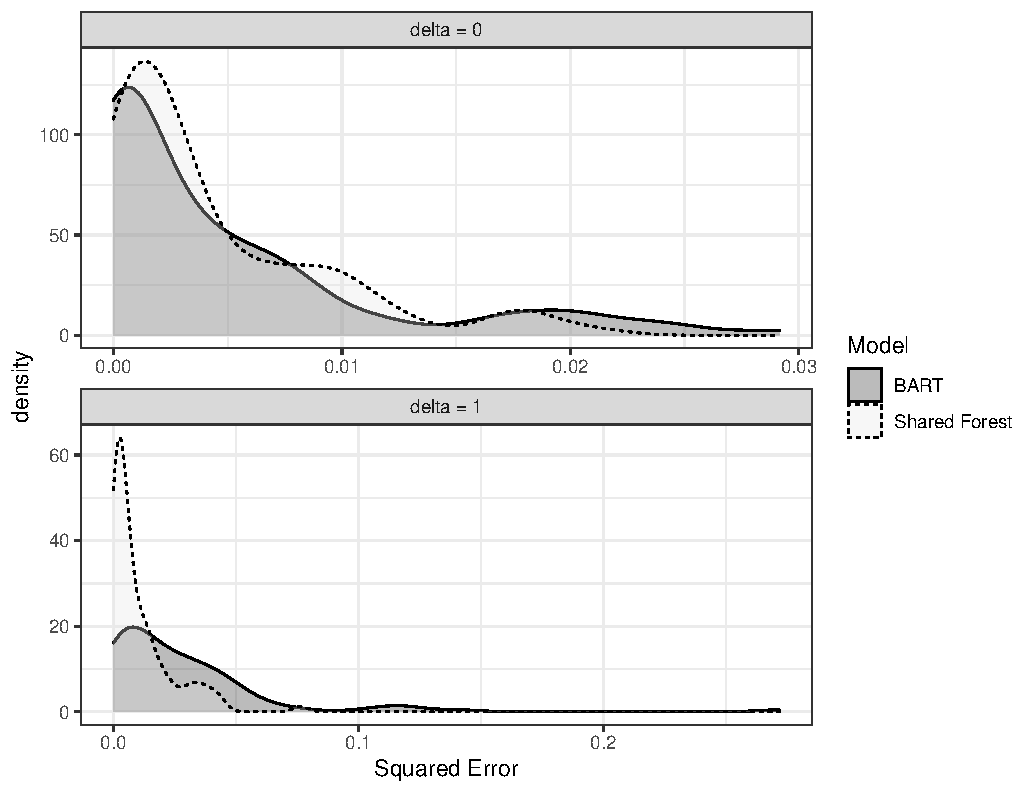
\includegraphics[width = .9\linewidth]{continuous_sim_results.pdf}
\end{frame}

\begin{frame}{Predicting $E(Y^* \mid \delta^*)$ }

% latex table generated in R 4.0.5 by xtable 1.8-4 package
% Tue Mar  1 10:17:05 2022
\begin{table}[ht]
\centering
\begin{tabular}{rlrrr}
  \hline
delta & variable & MSE & L\_bound & U\_bound \\ 
  \hline
0 & BART & 0.004875 & 0.000004 & 0.023207 \\ 
  0 & Shared Forest & 0.004330 & 0.000007 & 0.017697 \\ 
  1 & BART & 0.028464 & 0.000042 & 0.119264 \\ 
  1 & Shared Forest & 0.010399 & 0.000011 & 0.041591 \\ 
   \hline
\end{tabular}
\caption{\label{tab:mse} Mean of the squared errors (across simulations) comparing the true $E(Y^* \mid \delta^*)$ to the estimated $\hat{E}(Y^* \mid \hat{\delta})$.}
\end{table}

\end{frame}

\subsection{Binary/Binary} 

\begin{frame}{Predicting $E(\delta_2^* \mid \delta_1^*)$ }
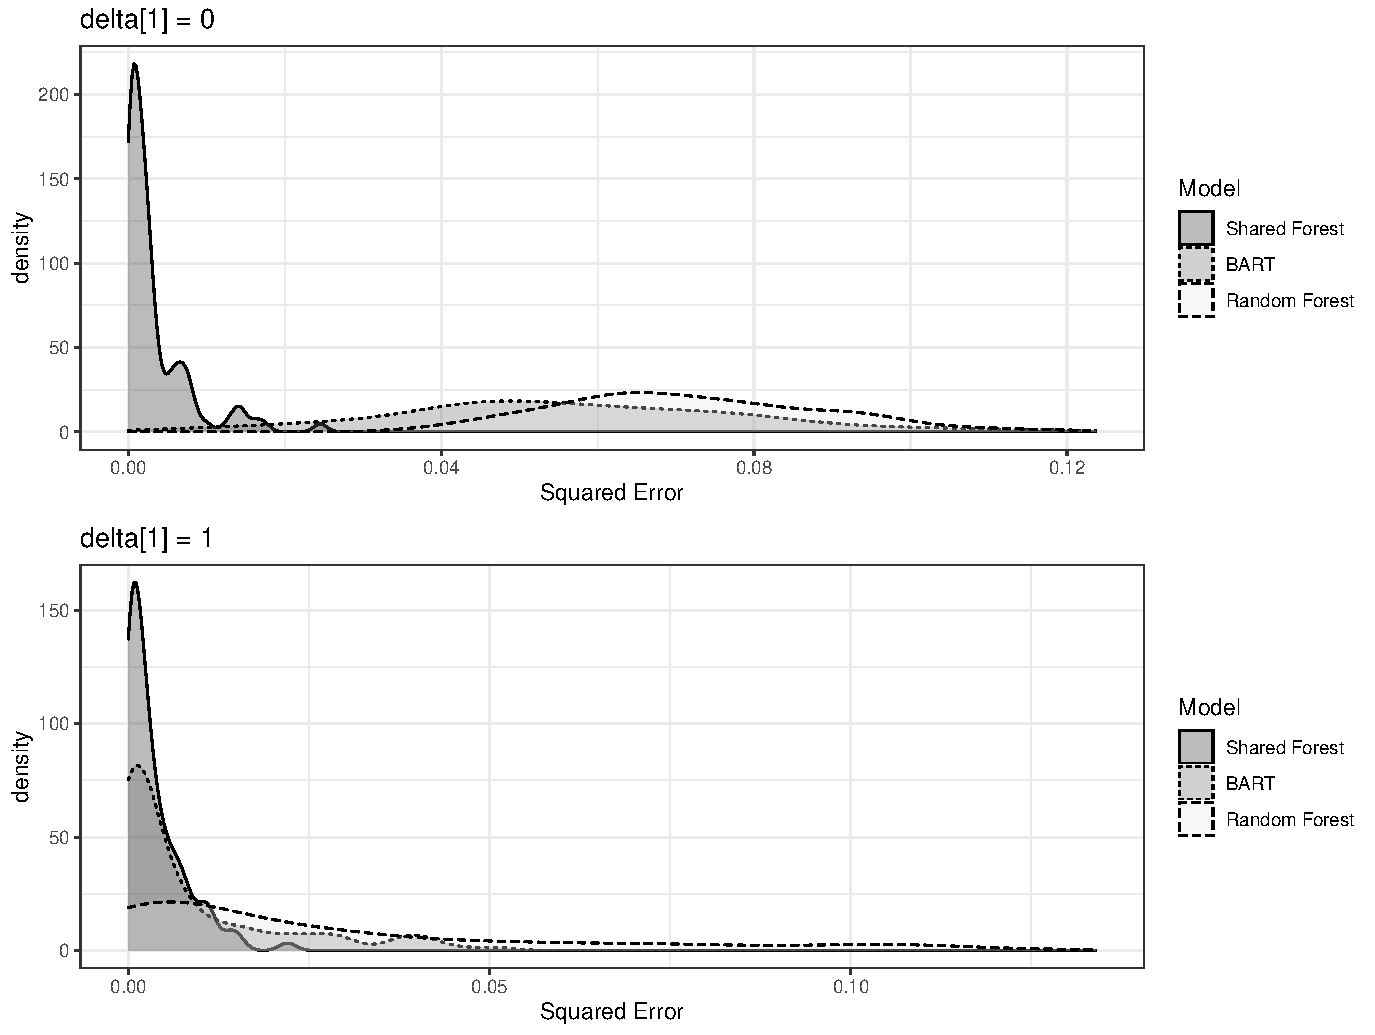
\includegraphics[width = .9\linewidth]{binary_sim_results.pdf}
\end{frame}

\end{document}